\documentclass{article}

\usepackage[top=1in,left=1in,bottom=1in,right=1in]{geometry}
\usepackage{graphicx}
\usepackage[absolute]{textpos}
\usepackage{lastpage}
\usepackage[hidelinks]{hyperref}
\usepackage[acronym,toc]{glossaries}
\usepackage{xspace}
\usepackage{tabularx} % for tables with line breaks
\usepackage{subfig}
\usepackage{relsize}

\usepackage{multibib}
\newcites{prod}{Products}
\newcites{ref}{References}



\newcommand{\Cyclus}{\textsc{Cyclus}\xspace}%

\newacronym{DRE}{DRE}{Dynamic Resource Exchange}

\makeglossaries


\title{Final Technical Report}


\begin{document}


\begin{titlepage}
%% 1. Identify the DOE award number; name of recipient; project title; name of
%%    project director/principal investigator; and consortium/teaming members.
  \begin{center}
    {\Large\bfseries Final Technical Report for Project DE-NE0000673}\\[1cm]
    {\huge\bfseries Market-Based and System-Wide Fuel Cycle Optimization}\\

    \vspace{2cm}
    {\bfseries Principal Investigator: Paul P.H. Wilson}\\[5pt]
    University of Wisconsin-Madison\\

    \vspace{2cm}
    Collaboratoring Investigator:\\[5pt]
    Anthony Scopatz, University of South Carolina\\
    \vfill

%% 2. Display prominently on the cover of the report any authorized distribution
%%    limitation notices, such as patentable material or protected data. Reports
%%    delivered without such notices may be deemed to have been furnished with
%%    unlimited rights, and the Government assumes no liability for the
%%    disclosure, use or reproduction of such reports.


    
  \end{center}
\end{titlepage}


\section*{Executive Summary}
%% 3. Provide an executive summary, which includes a discussion of 1) how the
%%    research adds to the understanding of the area investigated; 2) the
%%    technical effectiveness and economic feasibility of the methods or
%%    techniques investigated or demonstrated; or 3) how the project is otherwise
%%    of benefit to the public. The discussion should be a minimum of one
%%    paragraph and written in terms understandable by an educated layman.





\section{Introduction}

The goal of this project is to introduce optimization capabilities into the
\Cyclus{} fuel cycle simulator at two different levels of the simulation
capability.  

\subsection{\Cyclus{} Fundamentals}

\Cyclus{} is a nuclear fuel cycle simulation platform with a primary design
goal of flexibility to accommodate future innovations in nuclear fuel cycles.
This flexibility is achieved, primarily, through an agent-based paradigm in
which different models for agent behavior can be introduced through runtime
plugin modules.  The most important outcome of this paradigm is that new
behaviors can be introduced without having to change the fundamental platform,
thus allowing for better understanding of the impacts of those new behaviors.
Such new behaviors can represent different levels of fidelity for modeling
similar facilities, or entirely novel facilities that require different
modeling options.

A \Cyclus{} simulation consists of a deployment plan for a series of
facilities, possibly over many decades, with each facility represented by a
particular behavior model.  Each facility has a set of commodities that it
consumes and/or supplies, and a market for each commodity exists to facilitate
their exchange.  Commodities are traded in discrete quanta,
each of which has a specific quantitiy (often measured in mass) and a specific
quality (e.g. isotopic composition).  At each time step, consumers issue
requests for resources while suppliers issue offers of resources. A market
model uses some mechanism to determine which requests will be matched with
which offers, and resources are exchanged among facilites.  A more complete
description of the \Cyclus{} platform, including some of the work described
here, can be found in Ref. \citeprod{cyclus_fundamentals}.

\subsection{Optimization Needs}

The first target of optimization is at the level of individual commodity
markets during each time step.  Fundamental to the design of \Cyclus is the
ability for different facilities (often referred to as agents) to trade
discrete quanta of resources in the nuclear fuel cycle.  Initial
implementations of \Cyclus relied on an omniscient market agent that would
collect all the offers and requests and use some algorithm to determine which
trades would take place.  While this did allow for market like behavior, it
did not allow for different agents to value the same discrete quantum of
material differently.  Market-level optimization was implemented in the form
of the \gls{DRE} with the primary purpose of supporting agent-based valuation
of indvidual resource bids, accounting for flexibility in the behavior of the
facility, and fungibility among isotopes within a particular commodity.  As
will be seen, this encapsulation of the resource bid valuation entirely within
each agent promotes the fundamental flexibility of \Cyclus.

By itself, the consumer-centric \gls{DRE} left one gap in the efficient
implementation of commodity markets: suppliers had no knowledge of how the
consumers would value their bids and therefore no ability to customize their
bids to the consumer.  This was rememdied by extending the contents of a
request for resources to also include a mechanism for suppliers to query the
consumers for the value of a particular offer, so-called objective function
callbacks.  One original aim that proved unrealistic was the introduction of
realistic economic value functions in the context of these callback functions.
The ability to define the value of a resource offer in purely economic terms
is an appealing notion.  However, there remains too much uncertainty in the
various components of the costs of most fuel cycle facilities and processes to
provide credible estimates of the economic value of any single resource offer.
As will be discussed, the implementation of the objective function callbacks
does not preclude the introduction of purely economic valuation, but none were
explicitly provided as part of this work.

The second target of optimization is at the level of an entire simulation.  A
single \Cyclus instance can simulate the deployment, interaction and
decommissioning of a set of facilities over time, and provide metrics for the
performance of those facilities as well as for the overall fuel cycle.  It is
frequently interesting, however, to find a particular set of deployment,
interaction and decommissioning characteristics that will optimize some
combination of those metrics.  Given the emergent behavior that can arise from
an agent-based simulation, stochastic optimization techniques are the best
choice.  A swarm-based algorithm was implemented and demonstrated on
representative nuclear fuel cycle transition scenarios.  This same algorithm
was then also used to explore the limitations of different modeling paradigms
in achieving the same optimum solution\citeprod{rwc_fleet}.  Finally, a nested
optimization was carried out to identify best hedging scenarios given the
likelihood of disruption in the fuel cycle during transition.

While economic valuation of individual resource offers at the market level was
not implemented, there is also interest in determining an economic/financial
metric for the performance of an entire fuel cycle, particularly during
transition.  Such a metric would permit system-level optimization that focused
entirely/primarily on the economic performance over time.  Some work was done
to consider the economic metrics for complete nuclear fuel cycles,
particularly during transition.

\subsection{About this Report}

This report documents the implementation, testing, characterization and
demonstration of each of these features.  Section \ref{section:market}
describes the \gls{DRE} and the addition of objective function callbacks.
Section \ref{section:system} describes the fundamental optimization capability
and two advanced demonstrations of its use in fuel cycle simulations.  



\section{Market-level Optimization}\label{section:market}

The original design of \Cyclus included a notion of markets that presumed a
universal objective function for ascribing a value to resources offered for a
trade.  All consumers would submit their requests and all suppliers would
declare what resources they were able to offer, and the market would apply
some algorithm to match offers with requests.  While it did provide a
capability of swapping market models, it quickly became apparent that this
solution presumes a universal function for ascribing value to individual
quanta of material, while different facilities would generally have very
different ways of assessing the relative value of different resource offers.

This section describes the capability that allows \Cyclus to match consumer
requests with supplier offers while remaining consistent with the fundamental
goals of the \Cyclus framework.  In particular, this capability must support
the following.

\vspace{1em}
\noindent\textbf{Flexibility}: In order to support a maximum level of
flexibility in \Cyclus, each agent must operate as a \textit{black box}, with
no assumed knowledge of the capabilities or current state of other agents.
This permits individual facilities to be represented by plugins that can be
swapped individually without imposing restrictions on other agents in the
system.  The market clearing mechanism must be able to accept any request for
resources, regardless of its ability to be satisfied by the system.

\vspace{1em}
\noindent\textbf{Fungibility}: Since different fissile nuclides can fill
similar roles in the fuel cycle, resource offers may differ in composition but
still satisfy the needs of the consumer.  The market clearing mechanism must
be able to accept any offer of resources, without judgement on whether or not
it meets the goals of the corresponding request.

\vspace{1em}
\noindent\textbf{Agency}: Given the prior two characteristics, the final
ability to determine the details of a specific request, a specific offer, or
which offer is the most suitable match to a specific request must rest solely
in the hands of the facilities making those requests and offers.  The market
clearing mechanism may not impose any problem-wide value judgement on the
transactions.
\vspace{1em}

A market clearing mechanism that satisfies these high level requirements,
known as the \gls{DRE}, was designed and implemented.  \ref{subsection:dre}
first discusses the conceptual design of the \gls{DRE}, followed by a formal
definition of this system as a mixed-integer linear program to solve a
modified network flow problem.  Different solvers were studied to assess the
trade-off between accuracy and efficiency.  A number of sample problems are
presented to demonstrate the capability of the \gls{DRE}.  A more
comprehensive treatment of the \gls{DRE} can be found in \citeprod{dre_paper}
and \citeprod{gidden_thesis}.  Although the \gls{DRE} provides the necessary
components for market clearing in \Cyclus, it does not lead to the most
computationally efficient results.  In particular, the \gls{DRE} does not
provide a mechanism for suppliers to tailor their offers to the specific
interests of the consumers, even if their behavior models would allow them to
do so.  \ref{subsection:callback} introduces just such a mechanism, also
allowing suppliers to ascribe differening values to different offers for use
in resolving the \gls{DRE}.

\subsection{Dynamic Resource Exchange}\label{subsection:dre}

\subsubsection{Conceptual Design}

At the conceptual level, the \gls{DRE} implements the following communication
cycle at each time step in a \Cyclus simulation:
\begin{enumerate}
\item All consumers broadcast their requests to all suppliers.  Each request
  describes the desired quantity and quality (isotopic composition).
\item Suppliers respond to each consumer request with an offer to supply
  material.  Each supplier has the agency to decide whether or not to respond,
  and if so, how to respond.  Each offer describes an available quantity and
  quality.
\item Consumers use their own valuation process to rank the offers using the
  notion of preference.
\item All preferences are collected to be solved by a system that maximizes
  the total preference in the system.
\item The solution identifies specific resource trades that are then carried
  out among the facilities/agents.
\end{enumerate}

A the heart of the \gls{DRE} is a the \gls{MTP} \citeref{even1975complexity}
which belongs to the network flow family of optimization problems. A network
flow problem is represented by a graph, $G(N, A)$, comprises nodes $N$ and
arcs $A$. If flow can occur between some node $i$ and some other node $j$,
then it flows along arc $(i, j)$. Given a graph instance, optimal flow between
nodes can be found provided \textit{objective coefficients} and
\textit{constraints}. \textit{Decision variables} for this optimization
problem comprise the optimal \textit{flow assignment}. If all decision
variables are linear, then the resulting formulation is termed a \gls{LP}. If
some decision variables are integer (e.g., binary), the formulation is termed
a \gls{MILP}.

Transportation problems model the flow of a commodity between source nodes and
sink nodes which can have supply and demand constraints. A more complex
transportation-problem formulation can support systems in which supply or demand
can be met by multiple commodities.  There is a unit cost $c_{i,j}^{h}$ for
commodity $h$ to traverse arc $(i,j)$. A supplier of commodity $h$ has a certain
supply capacity $s_i^h$ which cannot be surpassed and consumers of commodity $h$
have a certain demand level which must be met, $d_i^h$.

In the simplest extension from the single-commodity to multi-commodity
transportation problem, arc constraints for all commodities are combined,
i.e., there is a single capacity $u_{i,j}$ for a given arc $(i, j)$. A classic
application of this enhanced complexity deals with data networks. Multiple
classifications of data exist, but they all must traverse the same network
infrastructure. Accordingly, the infrastructure can only accommodate a certain
quantity of total flow among all communication types.

A number of adjustments are made to a canonical MTP to accommodate specific
features of a nuclear fuel cycle, transforming it into a so-called
\gls{NFCTP}.

\begin{enumerate}
\item 
\end{enumerate}

\subsubsection{Mathematical Formulation}


The formulation of the multi-commodity flow problem is shown in Equation
\ref{eqs:MCTP}, in which the solutions are the set of flows of each commodity
between each request-bid pair, $\{x_{i,j}^h\}$. Note the commodity
coupling in Equation \ref{eqs:MCTP_cap}.

%%% 
\begin{subequations}\label{eqs:MCTP}
  \begin{align}
    %%
    \min_{x} \:\: & 
    \sum_{i \in I}\sum_{j \in J}\sum_{h \in H} c_{i,j}^{h} x_{i,j}^{h}
    & \label{eqs:MCTP_obj} \\
    %%
    \text{s.t.} \:\: 
    &
    \sum_{i \in I} x_{i,j}^{h} \geq d_{j}^{h}
    & 
    \forall \: j \in J, \forall \: h \in H \label{eqs:MCTP_dem} \\
    %%
    &
    \sum_{j \in J} x_{i,j}^{h} \leq s_{i}^{h}
    &
    \forall \: i \in I, \forall \: h \in H \label{eqs:MCTP_sup} \\
    %%
    &
    \sum_{h \in H} x_{i,j}^{h} \leq u_{i,j}
    & 
    \forall \: (i, j) \in A \label{eqs:MCTP_cap} \\
    %%
    &
    x_{i,j}^{k} \geq 0
    &
    \forall \: (i, j) \in A, \forall \: h \in H \label{eqs:MCTP_x}
    %%
  \end{align}
\end{subequations}
%%% 


A number of specific modifications can be made to accommodate specific
features of the nuclear fuel cycle, including:
\begin{itemize}
\item portfolios of requests, $R$, and offers, $S$, that represent the
  fungibility of resources,
\item partitioning of the graph into individual commodities,
\item multiple constraints, $k \in K_{\{s,r\}}$, on indivdiual suppliers or consumers,
\item constraints that depend on the quality of the individual trade (e.g. SWU
  constraints), $a_{i,j}^k$, and
\item mutually exclusive requests, $\tilde{x_j}$, that must be fulfilled by a
  single supplier such that $x_{i,j} = \tilde{x_j} y_{i,j}$ (e.g all fuel
  assemblies should come from the same fuel fabrication facility).
\end{itemize}
This allows the \gls{MTP} to be redefined into a more problem specific
\gls{NFCTP} as shown in Equation \ref{eqs:NFCTP}.  A more detailed discussion
of these details is available in ref \citeprod{dre_paper}.

\begin{subequations}\label{eqs:NFCTP}
  \begin{align}
    %%
    \min_{x, y} \:\: 
    & 
    z \:\: = 
    \sum_{(i, j) \in A_p} c_{i,j} x_{i,j} 
    \: + 
    \sum_{(i, j) \in A_e} c^{\prime}_{i,j} y_{i,j} 
    & 
    \label{eqs:NFCTP_obj} \\
    %%
    \text{s.t.} \:\:
    &
    \sum_{(i, j) \in A_{p_r}} a^k_{i,j} x_{i,j}
    \: + 
    \sum_{(i, j) \in A_{e_r}} a^{k\prime}_{i,j} y_{i,j}
    \geq b^k_r 
    &
    \: 
    \forall \: k \in K_r,  
    \forall \: r \in R 
    \label{eqs:NFCTP_req} \\
    %%
    &
    \sum_{(i, j) \in M_{r}} y_{i,j} \leq 1 
    &
    \forall \: r \in R 
    \label{eqs:NFCTP_mut_req} \\
    %% 
    &
    \sum_{(i, j) \in A_{p_s}} a^k_{i,j} x_{i,j}
    \: + 
    \sum_{(i, j) \in A_{e_s}} a^{k\prime}_{i,j} y_{i,j}
    \leq b^k_s 
    &
    \: 
    \forall \: k \in K_s, 
    \forall \: s \in S 
    \label{eqs:NFCTP_sup} \\
    %%
    &
    \sum_{(i, j) \in M_{s}} y_{i,j} \leq 1 
    &
    \forall \: s \in S 
    \label{eqs:NFCTP_mut_sup} \\
    %%
    &
    x_{i,j} \in [0, \tilde{x_j}]
    &
    \forall \: (i, j) \in A_p
    \label{eqs:NFCTP_x} \\
    %%
    &
    y_{i,j} \in \left\{ 0, 1 \right\}
    &
    \forall \: (i, j) \in A_e
    \label{eqs:NFCTP_y}
    %%
  \end{align}
\end{subequations}
%%% 

With the introduction of mutually exclusive requests, this problem becomes a
\gls{MILP}, requiring more complex methods for a rigorous solution.

Another important feature of the \gls{NFCTP} is the introductoin of false
consumers and suppliers to ensure a feasible solution.  If the total requests
of any single commodity exceed the supply, the network flow problem will match
one consumer with the false supplier, and vice versa.  No resources are traded
along such arcs.  Instead, consumers matched with false suppliers simple
receive no response to their request during that itme step.

\subsubsection{Solution Engines}

The formulation of this problem in a classical linear programming
representation enables \Cyclus{} to draw on both the literature for this field
and the various software libraries that exist to solve such problems.  The
leading open source solution is the \gls{COIN-OR} project \citeref{COINOR} that
provides robust implementation of standard algorithms for solving both linear
programs and mixed integer linear programs.

\Cyclus{} includes layers of abstraction to translate from an agent-centered
resource exchange formulation that will be most natural to fuel cycle modelers
into a network-centered linear program formulation that facilitates the use of
standard algorithms for solution.  These abstraction layers also enable
developers to connect alternative solver algorithms and libraries.

Testing was carried out with a simple, so-called \textit{greedy} solver, in
addition to the \gls{COIN-OR} linear programming (Clp) solver and the
\gls{COIN-OR} branch and cut (Cbc) mixed integer linear programming solver.
The greedy solver guarantees a feasible solution but not necessarily an
optimal solution, by using a heuristic of matching the highest preference
request with its highest preference bid, and so on until everything is
matched, including matches with false consumers/suppliers.  These different
solvers were tested to develop an understanding of their behavior in a number
of configurations.\citeprod{gidden_thesis} In addition to the overal computational
performance of the different solvers, there was also interest in understanding
under what circumstances the solvers achieved similar solutions.  These
results were measured as a function of the total number of requests and/or
offers in the system.  In some cases, calculated preference for individual
trades included stochastic components to introduce variability into the
simulations.  In these cases, large numbers of distinct realizations were
performed to study the mean behavior of the \gls{DRE}.

A sample of the results in shown in Figure \ref{fig:solver_comparison}.  This
problem has many reactors, each requesting fresh fuel for period reloads.  In
the reference case, the reactors are requesting invidivual assemblies rather
than batches of assemblies and trade preferences are adjusted based on a model
for relative facility location that allows for fine adjustment.  Three
different fuel cycle configurations were tested. In each case, the x-axis
shows the deviaiton in the achieved value of the objective function being
optimized by the \gls{DRE} while the y-axis shows the deviation in simulation
time.  The greedy solver is generally much faster, but does not achieve the
same level of optimization.  It is noteworthy, however, that the difference in
value of the objective function is not a perfect indicator of the differences
in the flows achieved by this solution.  Very similar flows may have different
objective function values.  A richer and more comprehensive analysis is
offered in Ref. \citeprod{gidden_thesis}.

%% include Gidden PhD figure 4.33 \label{fig:solver_comparison}

\subsubsection{Demonstration Problems}

A number of computational experiments are conducted to highlight unique
features enabled by the \gls{DRE} in Cyclus. Each experiment is performed by
solving instances of the \gls{DRE} using both the greedy heuristic solver and
to optimality with the branch-and-bound solver \gls{COIN-OR} Cbc solver. A
UOX-MOX one-pass recycle system with all required fuel cycle facilities is
taken as the base case scenario in order to reduce the complexity of the fuel
cycle and highlight departures from available simulators. For simplicity of
demonstration, reactors are assumed to refuel completely with a single
commodity rather than a combination of fuel types as is done in practice. A
simulation time frame of 50 years is chosen with one-month time-steps
(totaling 600 simulation time steps), sufficient to display all relevant
effects. The nominal parameters of all common facilities in the simulation are
shown in \citeprod{dre_paper}.

The base case scenario is not process constrained (i.e., it is constrained only
by the dynamics of Pu availability in the recycling stream). Reactors are
allowed to be fueled by either UOX or MOX, with a preference for MOX over UOX,
and refuel one-third of their total core mass every 18 months. Spent UOX fuel is
allowed to be recycled, whereas spent MOX fuel is sent directly to a
repository. In order to involve dynamism in the simulation, the population
reactors grows linearly over time at a rate of 1 reactor every 5 years. An
initial population of 20 reactors are deployed individually in each of the first
20 time-steps of the simulation as shown in Figure \ref{fig:deploy}. Note that
deployments are staggered in the initial period in order to avoid supply/demand
clustering effect. A diagram of the full base case fuel cycle is shown in Figure
\ref{fig:base}.

\begin{figure}
  \begin{center}
    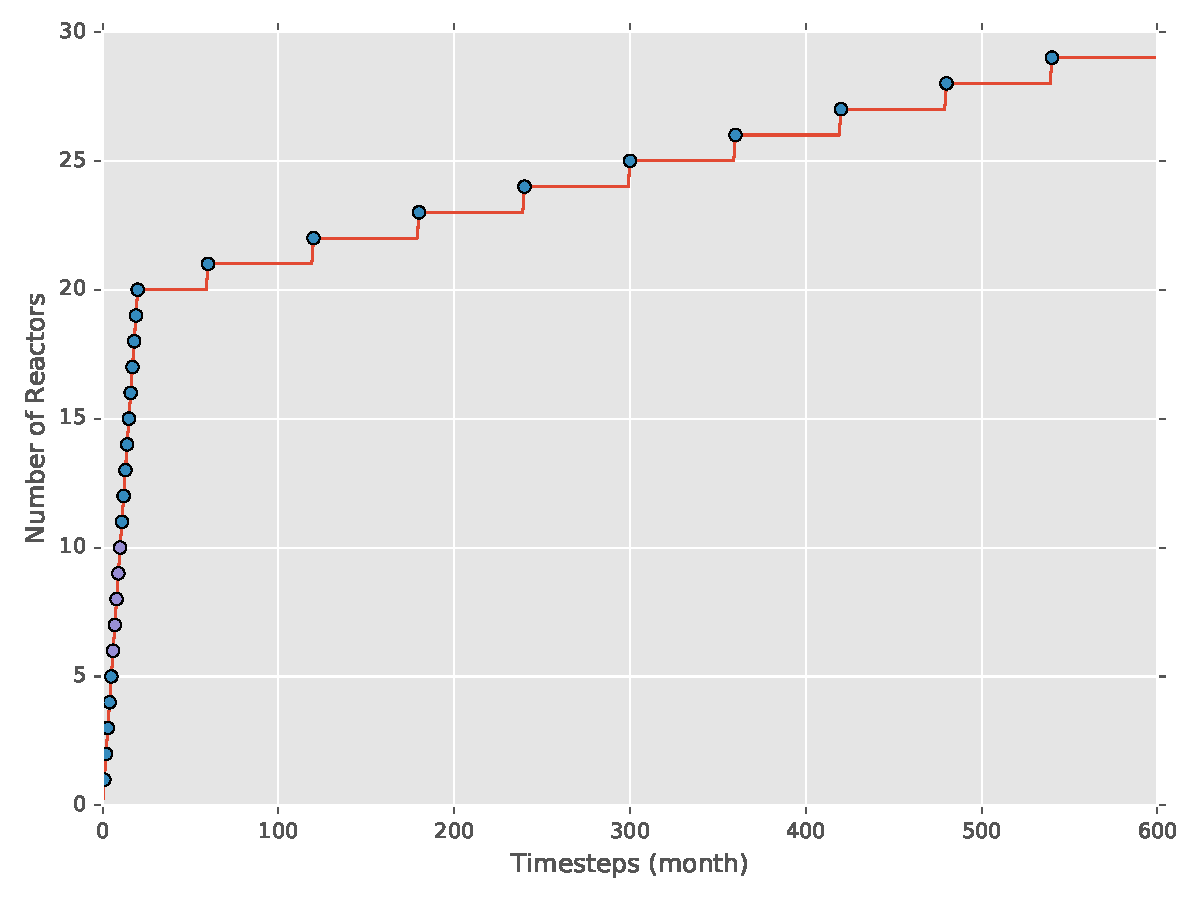
\includegraphics[width=0.75\columnwidth]{rxtr_deploy.pdf}
    \caption[]{
      \label{fig:deploy}
      Reactor deployment in each simulation as a function of simulation time
      steps. Each point in the graph is a reactor being deployed in the
      simulation. Deployments for the tariff scenario are distinguished by
      color: blue represents deployments in Region A and purple represents
      deployments in Region B.}
  \end{center}
\end{figure}

\begin{figure}
  \begin{center}
    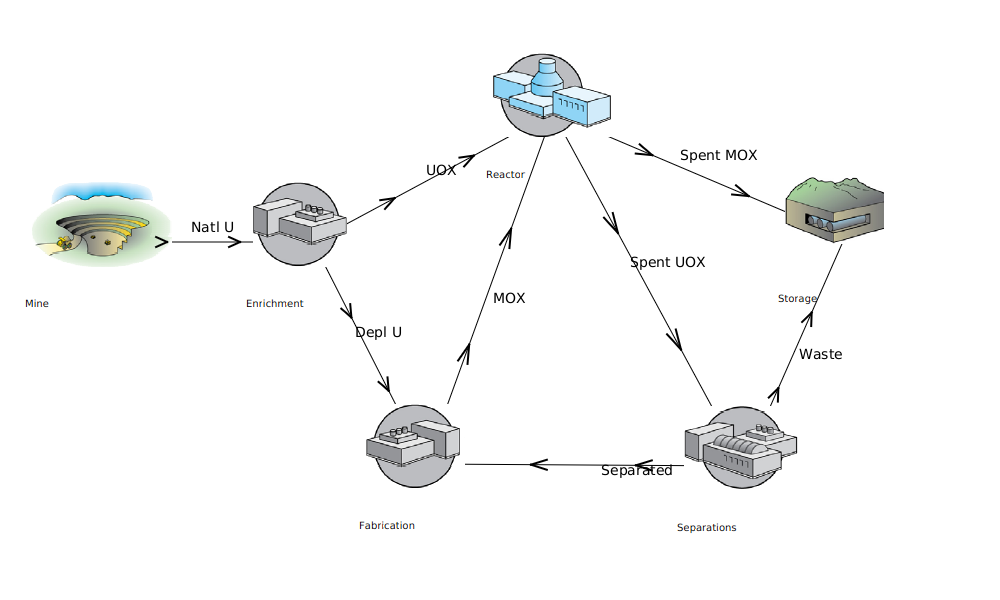
\includegraphics[width=0.75\columnwidth]{base_case_fc}
    \caption[]{
      \label{fig:base}
      Material routing between in the base case scenario, single-pass MOX fuel
      cycle. Possible arc flows are labeled with commodity names.}
  \end{center}
\end{figure}

Three perturbations from the base case scenario are used to provide examples of
modeling capability enabled through the use of the DRE. The scenarios are
summarized in Table \ref{scenarios} below and described in more detail in the
following sections. 

\begin{table}[]
\centering
\caption{Short Descriptions of Scenarios Ran}
\label{scenarios}
\begin{tabularx}{\textwidth}{|p{1.5cm}|p{1.5cm}|X|X|}
\hline
\textbf{Scenario  Name} & \textbf{Scenario Handle} & \textbf{Primary Departure from Base Case}                & \textbf{Capability Highlighted}                             \\ \hline
Separations Outage      & outage                   & Separations facility halts operation mid-simulation      & System flexibility to recycling facilities operation        \\ \hline
External MOX Supplier   & external                 & An additional supplier of MOX enters mid-simulation      & System flexibility to entry and exit of commodity suppliers \\ \hline
Regional Tariffs        & tariff                   & Two regions are modeled with dynamic trade relationships & Ability to model nontrivial international relationships     \\ \hline
\end{tabularx}
\end{table}

The first perturbation shows how the \gls{DRE} allows the system to respond to
arbitrary changes in the state of any facility.  In this case, the separations
facility shown in Figure \ref{fig:base} suffers an outage from $250 \leq t
\leq 300$, during which all other facilities continue to engage in trade,
adapting their trades for the available material.  The second perturbation
demonstrates how the \gls{DRE} can easily adapt to new facilities entering the
scenario.  An external source of MOX enters the simulation at $t = 250$ and
continues until it is exhausted.  The last perturbation demonstrates the
ability of agents to change their preference assignment algorithm dynamically
within the simulation.  In this case, it also engages the \gls{RIF} hierarchy
built into \Cyclus{} that allows for facilities to be owned by an
\textit{institution} that operates in a geopolitical \textit{region}, each of
which can influence how preferences are determined.  In this case, a second
region is added and a tariff is imposed on trade between the regions at $150
\leq t \leq 300$.

Importantly, in all cases, the only changes necessary to perturb the system
are local to the facility experiencing the perturbation.  All other
facilities, if properly configured to take advantage of flexibilities in the
base case, will automatically respond.  As such, these perturbations represent
much larger potential changes that can be introduced, either dynamically or by
user input into a fuel cycle.

A summary of the results is shown in Figures \ref{fig:uoxflow} and
\ref{fig:moxflow}.  Figure \ref{fig:moxflow} showcases the cumulative flow of
MOX fuel into all reactors as a function of simulation time step. Because
reactors can be fueled only with UOX or MOX, it represents the inverse of
Figure \ref{fig:uoxflow}. For example, whereas the tariff scenario utilizes
the most UOX, it utilizes the least MOX for the same reasons. A number of
additional features can be observed in Figure \ref{fig:moxflow} dealing with
departures from dynamic equilibrium of the base case scenario. The
undershooting and then overshooting of MOX consumption in the outage scenario
is visible. During the outage, less MOX is consumed, but immediately after the
outage, excess MOX is consumed until there is a return to dynamic
equilibrium. Additionally, a reduction in the total amount of MOX (sourced
from recycled UOX) consumed is observed in the external scenario. This is due
to a reduction in the available recycled UOX supply during periods of external
MOX consumption. In short, for each reload of external MOX, the system loses a
future amount of recyclable UOX.  A more complete discussion can be found in
Ref \citeprod{dre_paper}.

\begin{figure}
  \centering
  \begin{minipage}{\textwidth}
    \centering
    \subfloat[UOX flow.]{
      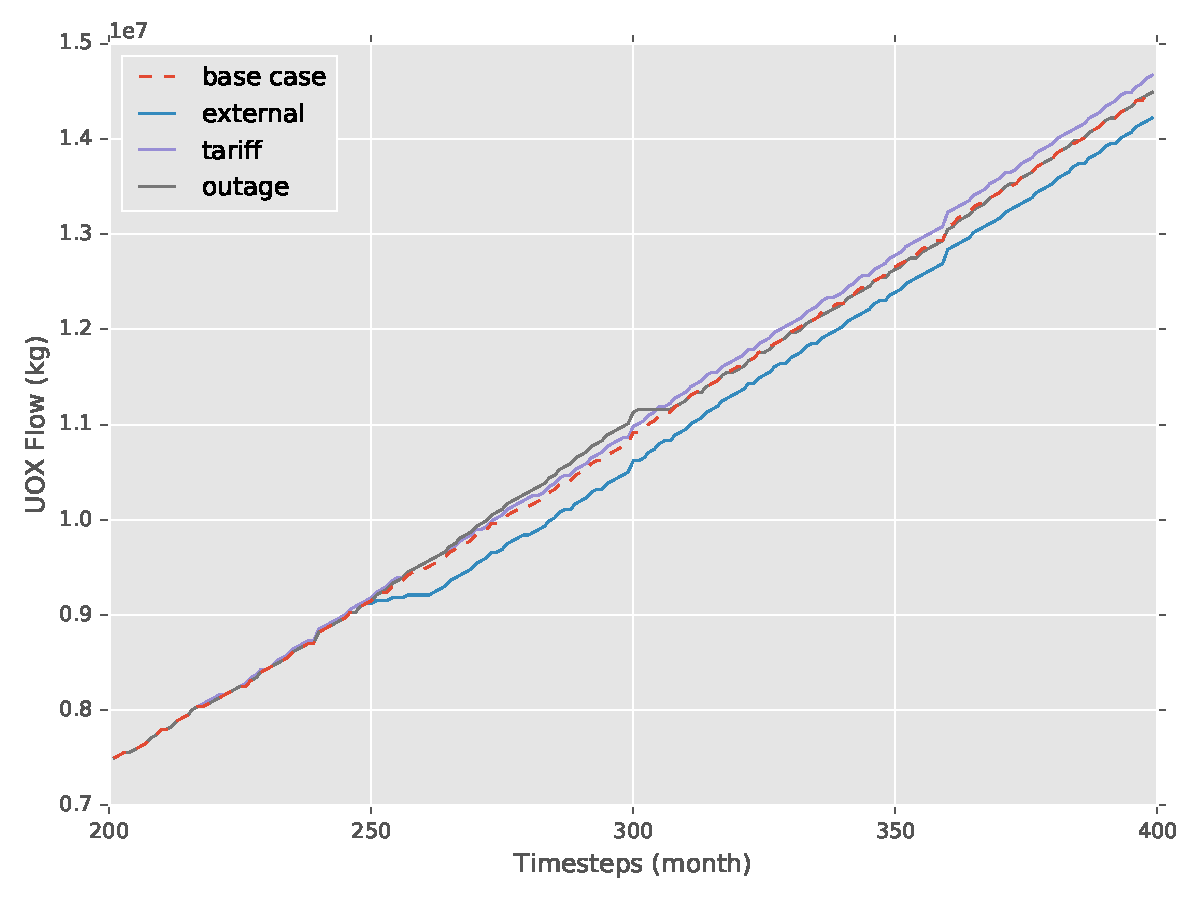
\includegraphics[width=0.5\textwidth]{uox_flow.pdf}\label{fig:uoxflow}}
    \subfloat[MOX flow]{
      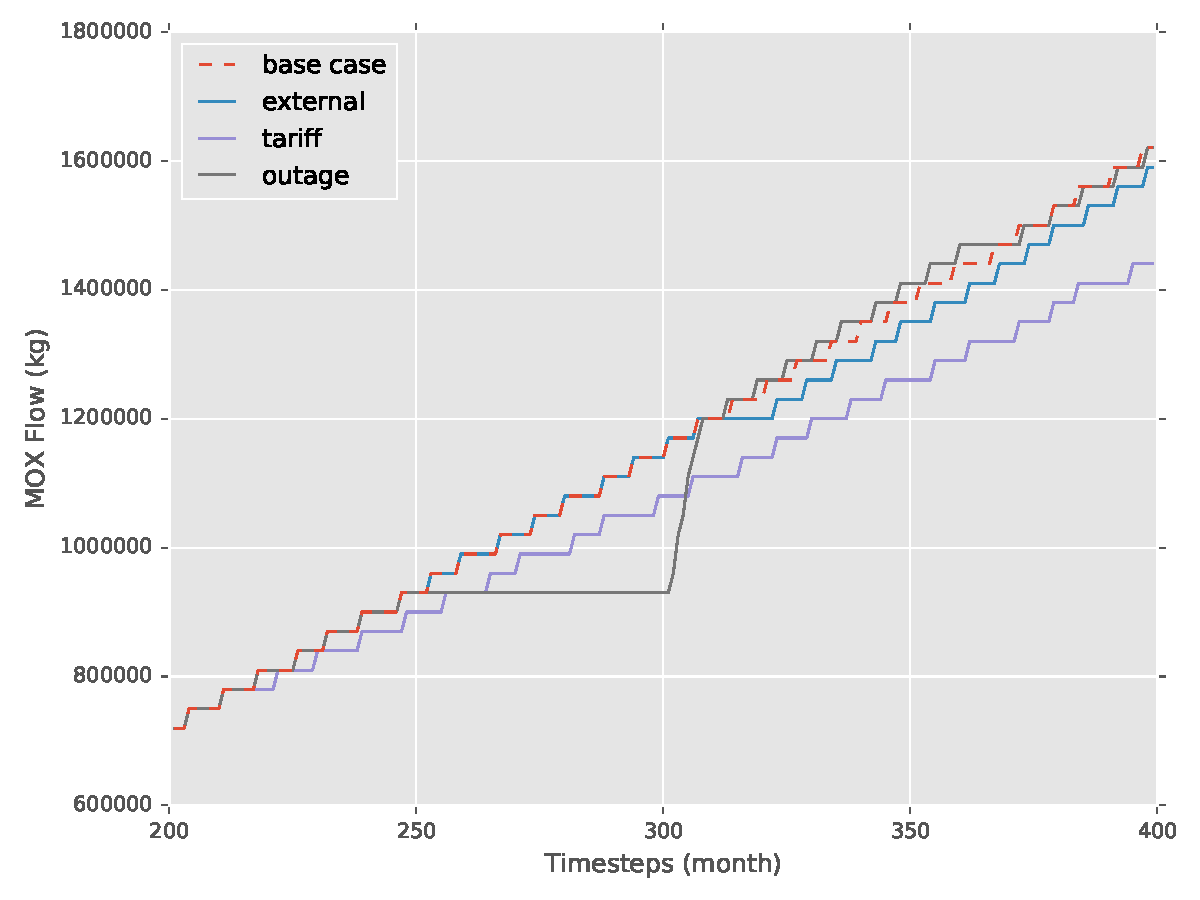
\includegraphics[width=0.5\textwidth]{mox_flow.pdf}\label{fig:moxflow}}
  \end{minipage}%
  \caption[]{
    \label{fig:flows}
    Cumulative flow of fuel in all Scenarios. The timestep period between 200
    and 400 is chosen to highlight all relevant transients. }
\end{figure}



\subsection{Objective Function Callbacks}\label{subsection:callback}

\subsubsection{Motivation}

As previously discussed, the basic implementation of the \gls{DRE} provides
the ability for consumers to evaluate different resource offers, but does not
provide the suppliers with any mechanism to judge how well those offers will
be recieved.  For suppliers that are unable to match the request exactly, but
otherwise have flexibility in the quantity and/or quality of the offers that
they issue, this leaves them essentially guessing which offers will be best
received by the consumer.  If the suppliers offers are poor matches, the
consumers may operate below their ideal performance or even experience supply
disruptions.  Three major types of remedy exist:
\begin{enumerate}
\item encourage supplier facilities to make many offers with different
  qualities/quantities,
\item increase the information included in a request to enable the supplier to
  make informed choices, or
\item provide a mechanism for the supplier to query the consumer.
\end{enumerate}

The first of these was ruled out because of the burden it would place of the
\gls{DRE} optimization algorithms.  Suppliers with continuously varying
paramter spaces might need to issue 1 or 2 orders of magnitude more offers for
each request in order to ensure that they were well-matched to the consumers
preference.  Since the performance of the \gls{DRE} scales with the number of
request-offer pairs, this would increase the time to resolve the market even
though the number of material flows wuold not change.

The second of these was ruled out because of the burden it would violate the
\Cyclus{} principle that each agent should operate as a black box to ensure
flexibility.  As each new piece of information is added to the request, all
agents would need to implement algorithms that could use that information to
guide their responses.  

This leaves the preferred solution of extending the request once to include a
function pointer that can be used by the supplier to query the consumer, in
which each consumer is free to respond to this query with as much complexity
as they require.


\subsubsection{Implementation}

Two small changes were made to give suppliers more control over the nature of
their offers and their interaction with the \gls{DRE}.  First, the contents of
a bid were expanded to include the supplier's preference for each bid.  This
information can then be used by consumers to impact their algorithm for
determining the ultimate request-bid preference.  As with the consumer's
ability to establish preference, the supplier is free to use any algorithm to
establish this preference.

The objective function callbacks have also been implemented, simply by
extending the contents of a request to include a pointer to a fcuntion with a
single argument of a single bid, and extending the interface with a function
that will return that pointer.  Suppliers are free to query the callback
function (or not) and implement any algorithm to use that information to amend
their bids.

Both of these changes require no changes to existing agent archetypes, unless
they want to take advantage of the new functionality.  A default bid
prefreence of 0 is assigned for all bids where it is not assigned explicitly,
so that all methods to generate bids will continue to function with no
changes.  Similarly, the callback functions are only queried if a supplier
archetype chooses to do so.


\subsubsection{Demonstration Problem}


This capability was demonstrated with a storage facility archetype that
determined its preference based in the specific decay heat of the offered
resource.  When added to the simulation, the archetype was configured with a
maximum specific decay heat and will never accept a material with a specific
decay heat above that threshold.  In addition, it will prefer materials with a
preference as high as possible below that threshold.

This archetype was used to fill multiple storage roles in a simulation that
also included a standard recipe reactor: wet storage with no maximum allowable
specific decay heat, dry storage with a modest maximum allowable specific
decay heat, and a geologic repository with a low maximum allowable specific
decay heat.  In such a simulation, the reactor, wet storage and dry storage
always offer their material to be taken by one of the other facilities.

There are a number of more subtle benefits of this approach.  These materials
can be offered in a single commodity market with no need to constrain the
possible flows \textit{a priori}.  If material happens to remain in wet
storage long enough that its decay heat drops sufficiently, its material can
be sent directly to the geologic repository.  All storage facilities
participate in the same market and only accept material that is suitable for
their characteristics.  In addition, intermediate storage facilities can trade
material based on its actual decay heat rather than its residence time.  Many
fuel cycle models rely on storage facilities with minimum residence times to
approximate the notion that spent-fuel transport and acceptance is typically
limited by its decay heat (among other related characteristics).  In this
case, the archetype can make decisions based on the operational characteristic
that matters rather than an approximate surrogate.

The preference function of the consumer always ensures that material only
flowed when the decay heat is sufficiently low.  In the absence of objective
function callbacks, however, the intermediate storage facilities would offer
all the resources in their inventory during every time step.  This would
result in many superfluous offers that exceeded the decay heat limits of the
consumers.  By using a callback function to probe the preference of the
receiving facility for each possible offer, it can avoid making offers that
are not going to be accepted by the receiving facility.

 


\section{System-level Optimization}\label{section:system}

The majority of fuel cycle analysis effort involves users running single
simulations defined primarily by the deployment history of various facilities
over time.  In some cases, users may manually alter those deployment histories
to meet some objective, iterating until they find the best possible outcome.
In fewer instances, that iteration has been automated to seek optimal
solutions (e.g. \citeref{hays}).  By modeling discrete facilities over 1 month time
steps, \Cyclus{} offers many degrees of freedom for defining the deployment
history of its facilities, underscoring the value in an automated optimization
system.

This task focuses on the design, implementation and testing of a system that
uses \Cyclus{} to find optimal deployment histories within the bounds of
specific fuel cycle scenarios.  The first section defines a reference fuel
cycle scenario to be used when developing a system for fuel cycle
optimization.  The following section discusses the development of the basic
optimization system, including the choice of optimization algorithm and the
structure of the decision space.

This capability was then extended to seek an optimum deployment strategy under
the possibility of disruption of the fuel cycle at some future time.  The
methodology employed for this work used the same optimization algorithm, but
added nested layers of optimization to identify a hedging strategy that
minimizes the impact of a disruption during the transition.

\subsection{Reference Problem Description}

The EG23 transition defined by the Fuel Cycle Options campaign provided a
convenient problem for studying the optimization of fuel cycle scenarios.
This scenario starts with 100 \gls{LWR}s and follows an exponential growth of
  1\% per year for 200 years, while transitioning to a fuel cycle based
  entirely on \gls{SFR}s.  Plutonium from the separations of \gls{LWR} fuel is
  used to start the \gls{SFR} fleet, transitioning to recycling of their own
  fuel in the long term.  The deployment history of \gls{LWR} separations
  capacity is fixed, and reactor deployment history is to be optimized.  The
  goal is to complete the transition, defined by the decommissioning of the
  last \gls{LWR}, as quickly as possible.  More details of this transition are
  available in Ref. \citeprod{rwc_fff}.


  
\subsection{Optimization Design, Implementation and Demonstration}

\subsubsection{Requirements and Algorithm Options}
Using a fuel cycle simulator as part of an optimization objective is a
challenging problem for several reasons:

\begin{itemize}
\item The objective function is generally not a linear function of input
  parameters.
\item No derivative information for the objective is available.
\item The objective function may be discontinuous.
\item Input variables to the objective function may be discrete.
\item The input parameter space could be large necessitating constraints
  for reasonable performance.
\item The objective function may be stochastic - i.e. different runs with
  the same inputs may produce different outputs.
\item The objective function is expensive to evaluate - seconds to minutes
  for a single iteration.
\end{itemize}

This kind of problem is often referred to as black-box\footnote{While this use
  of ``black box'' is functionally different than the usage in Section
  \ref{section:market}, it is based on the same notion that there is no ability to
  have internal knowledge of the system.}  optimization. Another challenge is
desirability of the optimization process to be effective over many different
simulation scenarios. There is no single, well-defined objective to be
optimized.

There are several classes of algorithms for addressing block-box optimization
of this nature:
\begin{itemize}
\item \textbf{Pattern Search} algorithms expand and contract their search over
  a discretized decision space, with convergence governed by the rates of expansion and
  contraction.
\item \textbf{Swarm} algorithms follow the trajectories of a set of search
  points through the decision space, with the velocities of those points
  determined by the location and magnitude of the objective function at each
  evaluation.
\item \textbf{Evolutionary} algorithms evaluate the objective function across
  a population of points sampled from the decision space, and then look at
  ``genetic'' combinations of the best available points to identify better
  possible points.  Mutations can be used to modify the search process.
\item \textbf{Surrogate} algorithms form an approximate model of the objective
  function over the decision space, often of a form that can be optimized with
  algorithms that rely on information note available from the black-box
  approach.
\end{itemize}

In order to test these algorithms with the reference EG23 problem, it is
necessary to define the decision space and objective function.

\subsubsection{Decision Space Formulation}

Conceptually, the decision space is defined by the number of reactors of each
variety being deployed at each time step, with the total capacity constrained
to match the total electricity growth rate.  A naive implementation based on
this conceptual problem results in unbounded decision variables in a space
bounded by explicit constraints.  Many black-box algorithms are challenged by
such a decision space, resulting in evaluations of infeasible solutions (those
outside the constraint) that are then penalized in the evaluation of the
objective function because of they are outside the constraint.  It is
therefore preferable to develop a formulation with a bounded decision space,
in which the constraints are represented by the bounds of the decision
variables.

The decision space for one such formulation is defined by the fraction of
capacity additions at each time step that will composed of each reactor type.
Each decision variable is then bounded on the interval $[0,1]$.  Furthermore,
by selecting the fraction of each reactor type in succession, and updating the
bounds for the next reactor type after each selection, the entire search space
is accessible without violating the constraint.

These fractions can be converted to the number of reactors as shown in
Equation \ref{eqn:transform-reactors}.

\begin{equation}
    N(t, r) =
    \begin{cases}
        floor\left(\frac{
            \mathlarger{V_{fac}(t,r) \cdot \left[P_{new}(t) - \sum\limits_{r'=1}^{r-1} N(t,r') \cdot C(r')\right]}
        }{\mathlarger{C(r)}} + 0.5\right) & : r > 0 \\
        floor\left(\frac{
                \mathlarger{P_{new}(t) - \sum\limits_{r'=1}^{r_{last}} N(t,r') \cdot C(r')}
        }{\mathlarger{C(r)}} + 0.5\right) & : r = 0
    \end{cases}
    \label{eqn:transform-reactors}
\end{equation}

$N(t, r)$ is the number of reactors of type $r$ to deploy at time $t$,
$floor(x)$ is the closest integer to $x$ that is less than or equal to $x$,
$V_{fac}(t,r)$ is the decision variable value for facility $r$ at time $t$,
$P_{new}(t)$ is new capacity to be deployed at time $t$, and $C(r)$ is the
power capacity for a single reactor of type $r$ (e.g. 1000 MWe). The
$N(t,r=0)$ deployments must be computed after all $N(t, r > 0)$ deployments.
Reactor type $r=0$ is used to deploy any remaining new power capacity that is
not satisfied by the other reactor types.

\subsubsection{Objective Function}

Many possible objective functions can be used to assess fuel cycle
transitions, and selecting objective functions is an area of study in its own
right (in addition to defining them with sufficient certainty to be useful).
The objective function was designed to drive toward a fast-reactor-only fuel
cycle as quickly as possible while simultaneously discouraging/penalizing
unfueled reactors.  Because fast reactors are fueled only with recycled
fissile material, it is possible for some deployment schedules to cause fast
reactors to idle without fuel.  The objective function used is shown in
Equation \ref{eqn:obj}.

\begin{equation}
    \label{eqn:obj}
    O_{sim} = \frac{\sum\limits_{t \in sim} E_{t,\;LWR}}{\sum\limits_{t \in sim} E_{t,\;tot}}
\end{equation}

$O_{sim}$ is the objective function value for an entire simulation,
$E_{t,\;LWR}$ is the energy produced by all \gls{LWR}s in time step $t$, and
$E_{t,\;tot}$ is the energy produced by all reactors in time step $t$.
Because the optimizer is trying to minimize the objective value, more
\gls{LWR}s results in a larger numerator (a worse objective value), and
unfueled fast reactors shrinks the denominator (also a worse value).  It is
notable that this objective function does not penalize unfueled reactors very
heavily relative to the penalty for \gls{LWR} energy.  This is intentional and
allows the optimization to explore potentially interesting trade-offs related
to expediting the transition.


\subsubsection{Master-worker implementation}

As black box techniques, all of the optimization algorithm classes explored
here rely on a large number of independent evaluations of the objective
function.  After the optimization algorithm selects the set of decision
variables for each evaluation, an objective function evaluation consists of a
\Cyclus{} simulation followed by some post-processing of the results.
Depending on the algorithm there were $O(200)$ evaluations per iteration, with
$O(300)$ iterations, for a total of $O(60,000)$ evaluations.  

The optimization system for \Cyclus{} was developed using a master-worker
paradigm in a high-throughput computing environment.  For each iteration, the
optimization algorithm ``master'' would assign work, in the form of a
\Cyclus{} input file, to a set of independent ``workers'', each of which would
run \Cyclus{} and evaluate the objective function based on the output.  Such a
system is flexible to the number of available workers at any time, and multiple
masters can share the same pool of workers.  Such a system allowed a thorough
exploration of the different algorithms, with over 700,000 \Cyclus{}
evaluations used for the final comparison.  Development and testing relied on
about 1 million additional \Cyclus{} evaluations, consuming about 30,000 CPU
hours over 7 days.

\subsubsection{Algorithm Selection and Sample Results}

A variety of open source libraries, each implementing algorithms in one or
more of the classes of optimization algorithms, were tested for their
performance using the reference problem described above.

The overhead and time involved in dispatching and running \Cyclus{} simulations
is much larger than the time and computational resources required to run the
each optimizer itself. Because of this, the optimizers are compared by
primarily looking at the best objective function value achieved as a function
of the total number of objective function evaluations.  Table
\ref{tab:exp1-summary} summarizes the results for all runs done with each
optimizer.  Only a single run was performed with the DIRECT algorithm because
it is deterministic and multiple runs on the same problem will always give the
same result.  The optimizers are listed in order of performance/effectiveness
with PSwarm being the best performer and DIRECT being the least effective.

\begin{table}[h]
    \centering
    \begin{tabular}{ |r | c c c c| }
        \hline                       
                      & Run & \# evaluations & \# iterations & Best objective \\
        \hline                       
        PSwarm          & 1 & 60,046 & 356            & 0.1704 \\
        PSwarm          & 2 & 60,062 & 349            & 0.1670 \\
        PSwarm          & 3 & 60,153 & 349            & 0.1671 \\
        PSwarm-biannual & 3 & 62,022 & 368            & 0.1423 \\
        JEGA            & 1 & 28,029 & 246            & 0.1884 \\
        JEGA            & 2 & 59,203 & 518            & 0.1848 \\
        JEGA            & 3 & 26,821 & 236            & 0.1889 \\
        HOPSPACK        & 1 & 60,012 & $310^\text{*}$ & 0.2816 \\
        HOPSPACK        & 2 & 59,840 & $310^\text{*}$ & 0.2637 \\
        HOPSPACK        & 3 & 59,956 & $310^\text{*}$ & 0.2900 \\
        SCOLIB EA       & 1 & 60,048 & 402            & 0.4742 \\
        SCOLIB EA       & 2 & 60,048 & 402            & 0.4871 \\
        SCOLIB EA       & 3 & 60,048 & 402            & 0.4871 \\
        SCOLIB DIRECT   & 1 & 58,260 & 16             & 0.5531 \\
        \hline                       
    \end{tabular}
    \captionsetup{justification=centering}
    \caption[Summary of optimizer performance]{

        Summary results for all optimizer runs. The additional
        \emph{PSwarm-biannual} run is identical to the other PSwarm runs
        except it had bi-annual instead of annual deployments resulting in
        only 200 optimization variables. \\
        
        \hspace{\textwidth}
        
        * The HOPSPACK optimizer did not have well-defined iteration
        boundaries.

    }
    \label{tab:exp1-summary}
\end{table}


The PSwarm and JEGA solvers were the strongest performers, with PSwarm beating
out JEGA slightly in both convergence rate and best solution found.  The other
solvers performed unsatisfactorily.  Figure \ref{fig:exp1-converge} provides a
good picture for roughly evaluating how each optimizer performed with respect
to the following criteria:

\begin{enumerate}

    \item How good was the best objective value found?

    \item How quickly did the optimizer converge toward a good solution?

    \item How consistently does the optimizer perform on criteria 1 and 2 over
        multiple runs and/or problems?

\end{enumerate}

In addition to the runs for each optimizer described above, Table
\ref{tab:exp1-summary} and Figure \ref{fig:exp1-converge} contain data from
one additional run using the PSwarm optimizer with bi-annual deployments
instead of annual deployments.  More detailed discussion of each result is
available in Ref. \citeprod{rwc-dissertation}.  The PSwarm optimizer was selected as
the primary optimization algorithm for the \Cyclus optimization system.

\begin{figure}
    \centering
    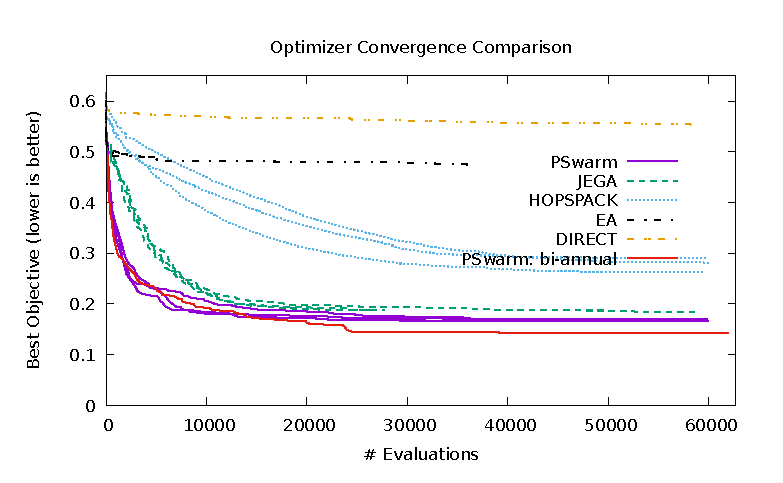
\includegraphics[width=1.0\textwidth]{converge.eps}
    \captionsetup{justification=centering}
    \caption[Optimizer convergence curves]{Objective value convergence curves for all optimizer runs.}
    \label{fig:exp1-converge}
\end{figure}

Figure \ref{fig:exp1-bestfoundpower} shows both the total power and LWR power
generated over time for the best deployment schedule found among all runs.
Figure \ref{fig:exp1-bestknownpower} shows both the total power and LWR power
generated over time for the best deployment schedule found by the PSwarm
optimizer using smaller $\pm5\%$ bounds instead of $\pm10\%$ bounds around the
growth curve. This deployment schedule results in an objective value of
$0.1557$.  This is noticeably better than the best result by other
400-variable optimizer runs which was $0.1671$ from the PSwarm optimizer.  The
larger 10\% power curve bounds effectively result in a solution space
containing $[\frac{\text{new range}}{\text{prev. range}}]^{n}$ times as many
possible solutions as the 5\% bounds where range refers to the difference
between upper and lower bounds and $n$ is the number of variables in the
problem. So doubling the size of the bounds for this 400-variable problem
results in a solution space with $2^{400}$ times as many possible solutions --
much larger than before.

\begin{figure}
    \centering
    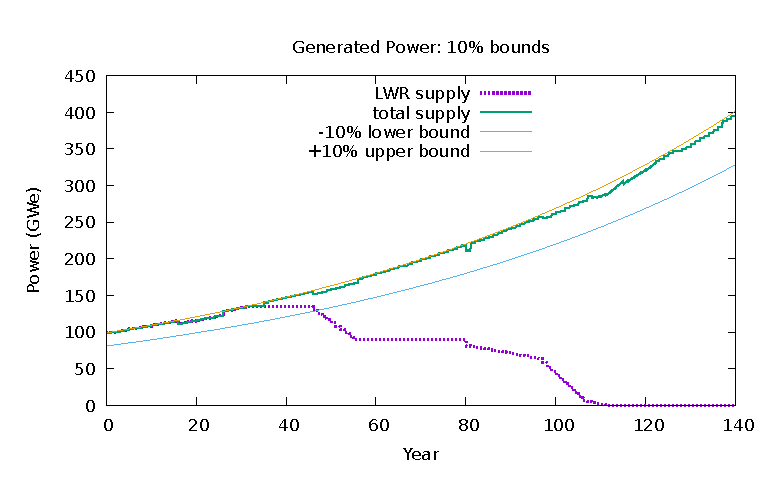
\includegraphics[width=0.75\textwidth]{best-found-power.eps}
    \caption[Power for best build schedule with $\pm10\%$ bounds]{ Both
      \gls{LWR} and total (\gls{SFR} and \gls{LWR}) generated power over time
      for the best deployment schedule found among all the primary
      optimization runs using the $\pm10\%$ bounds around the 1\% power growth
      curve and annual deployments.  }

    \label{fig:exp1-bestfoundpower}
\end{figure}

Figure \ref{fig:exp1-bestfoundpower} shows that the optimizer found a solution
near a corner of the parameter space, building along the upper power bound and
only building fast reactors as soon as they become available.  The solution
shown in Figure \ref{fig:exp1-bestknownpower} is similar in that it rides the
+5\% upper bound for nearly all of the 200 years.  The only significant
exception is a short period in the ~10 years leading up to fast reactor
availability in year 35. This makes sense - \gls{LWR} deployments are stopped
and the optimizer utilizes its 5\% flexibility to achieve a jump start in year
35 with a larger number of \gls{SFR} deployments than would otherwise have been
possible.  This allows the \gls{LWR}s to be phased out more quickly over all.

\begin{figure}
    \centering
    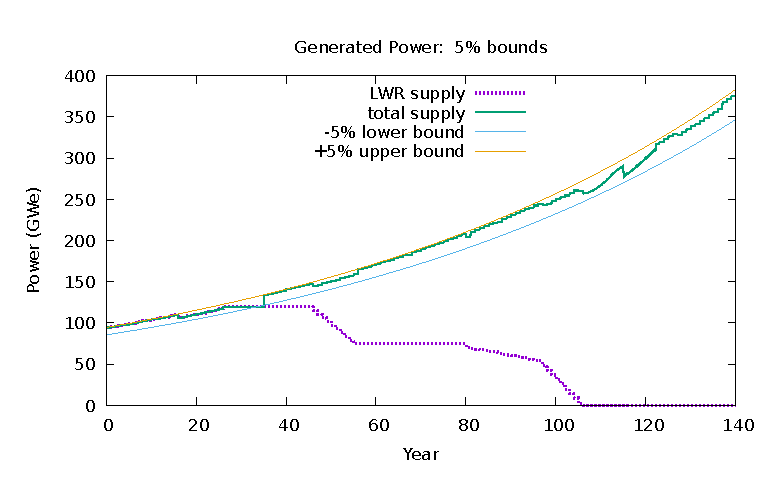
\includegraphics[width=0.75\textwidth]{best-known-power.eps}
    \caption[Power for best build schedule with $\pm5\%$ bounds]{ Both
      \gls{LWR} and total (\gls{SFR} and \gls{LWR}) generated power over time
      for the best deployment schedule found by the PSwarm optimizer using
      smaller $\pm5\%$ bounds around the 1\% power growth curve and annual
      deployments.  }

    \label{fig:exp1-bestknownpower}
\end{figure}

\subsection{Disruption Analysis and Hedging Strategies}
\subsubsection{Motivation}

When conducting transition analysis for nuclear fuel cycles, a fundamental
assumption is that the transition will proceed in an orderly fashion from the
current configuration until it is complete.  Transitions typically take over
100 years to become complete, and often longer.  Societal motivations and
needs are very likely to change over such time scale, probably leading to
changes in course for nuclear fuel cycle transitions, calling into question
this fundamental assumption.

The work under this task builds upon the system-level optimization to study
the response of the system to a disruption in the trajectory to a new fuel
cycle concept.  Many types of disruption are possible, from small changes in
the configuration of the systems being deployed during the transition, to
large changes in policy that render some key systems no longer usable.  Over
the time scales of interest, it is possible that there may be multiple
disruptions.  It is not generally possible to predict when such disruptions
will occur.

Nuclear fuel cycle transitions are often assessed according to a set of
performance metrics, where the best transition is determined by optimizing
against one or more of these metrics.  In the face of disruption, it may be
more valuable to identify a transition that will be impacted the least by such
a disruption.  Such a transition may not be optimal in the event that no
disruption occurs, but can have the highest likelihood of a near optimal
performance under the presumption of disruption.  The optimization system for
\Cyclus{} can be nested to identify such transitions, known as hedging
strategies since they hedge against the risk of disruptions.

\subsubsection{Methodology}

The previous section showed how to determine the optimum deployment history
for a given objective function and given scenario description.  While the
addition of a disruption changes the scenario, it is still possible to
identify an optimum for this new scenario.  However, the decision space of
such an optimization problem must be slightly different.  First, consider a
candidate deployment history, $D$, that will be subject to a disruption. All
histories must start on this path as they have no \textit{a priori} knowledge
if or when a disruption will occur.  After the introduction of a disruption at
time, $t_d$, an optimization analysis can occur to find the optimal deployment
history, $D'$, that must only differ from $D$ in the time period after the
disruption.  That is, the decision space for this optimization problem does
not include the decisions made prior to $t_d$.  We define $R^*(D,t_d)$ as the
optimum deployment history that begins as history $D$ but suffers a disruption
at time $t_d$, and $S^*(D,t_d) = O[R^*(D,t_d),t_d]$ as the value of the
objective function, $O(D)$, when deployment history $R^*(D,t_d)$ is evaluated
in a scenario in which a disruption occurs at time $t_d$.

Since the actual time of disruption is not known, we must assume a probability
distribution, $p(t_d)$, so that is finally possible to determine the hedging
score for a given initial deployment history, $D$, as:

$$H(D) \equiv \int_0^\infty S^*(D,t_d) \cdot p(t_d) dt_d,$$

\noindent which can be approximated as:

\begin{equation}
  H(D) \approx \sum_{i=0}^m S^*(D,t_i) \cdot p(t_i) \Delta t. \label{eqn:Happrox}
\end{equation}

Finally, this can be used as an objective function itself, to seek the initial
deployment strategy, $D$, that results in the optimum value of $H(D)$.


\subsubsection{Implementation}

Using this conceptual methodology directly requires many levels of optimization:
\begin{enumerate}
\item $O(10^5)$ evaluations of objective function $H(D)$
\item For each evaluation of $H(D)$, $O(10)$ evaluations of $S^*(D,t_d)$, and
\item For each evaluation of $S^*(D,t_d)$, $O(10^5)$ evaluations of objective
  function $O(D)$ in order to find $R^*(D,t_d)$.
\end{enumerate}

Given the limited ability to parallelize across the PSwarm algorithm (or any
black-box algorithm), this results in a currently unrealistic amount of
computational effort, even using the high throughput master-worker paradigm.
One way to reduce the effort is to introduce an approximation for
$S^*(D,t_d)$.  While the choice of such an approximation is an interesting
research topic itself, for the purpose of demonstrating the overall
capability, we chose the approximation:

$$S^*(D,t_d) \approx \frac{t_d}{t_{end}} O(D,t_d) + \frac{t_{end}-t_d}{t_{end}} O^*(t_d),$$

\noindent where $O^*(t_d)$ is the value of the objective function for the
deployment history that is optimum for a disruption at time $t_d$.  For a
discrete set of disruption times identified in Eqn \ref{eqn:Happrox}, each
$O^*(t_d)$ can be evaluated once \textit{a priori}.  Each subsequent
approximation of $S^*(D,t_d)$ requires only a single evaluation of the
objective function, $O(D)$.


\subsubsection{Problem Definition}

A variation of the EG23 transition analysis was used to demonstrate this
capability.  The presence of disruptions is likely to increase the chance that
reactors are idle after their deployment, so the objective function is
modified to introduce a penalty for such circumstances.

\begin{equation}
    O_{sim} = \frac{\sum\limits_{t \in sim} E_{t,\;LWR}}{\sum\limits_{t \in sim} E_{t,\;tot}}
              \cdot
              \frac{\sum\limits_{t \in sim} C_{t,\;tot}}{\sum\limits_{t \in sim} E_{t,\;tot}}
    \label{eq:exp3-obj}
\end{equation}

In this case, $C_{t,tot}$ is the total installed capacity; the lower the capacity factor, the higher the objective function.

\subsubsection{Disruption Details}

In order to focus on the methodology, a simple disruption was introduced in
the form of a 33\% reduction in the Pu available for fabrication of \gls{SFR}
fuel.  This could be interpreted as an approximation to a number of different
realistic scenarios, including a policy decision to shift away from breeders
and towards burners.

It is also necessary to introduce a probability distribution for the when the
disruption occurs.  In this case, a gamma distribution is chosen, and shown in
Figure \ref{fig:exp3-gamma-dist}.

\begin{equation}
    p(t_d) = \frac{600}{\Gamma(1.5)\cdot 2^{1.5}} \left(\frac{t}{600}\right)^{0.5} \mathlarger{e^{\frac{\mathlarger{\mathsmaller{-}t}}{600 \cdot 2}}}
    \label{eq:gamma-dist}
\end{equation}

\begin{figure}[!htb]
    \centering
    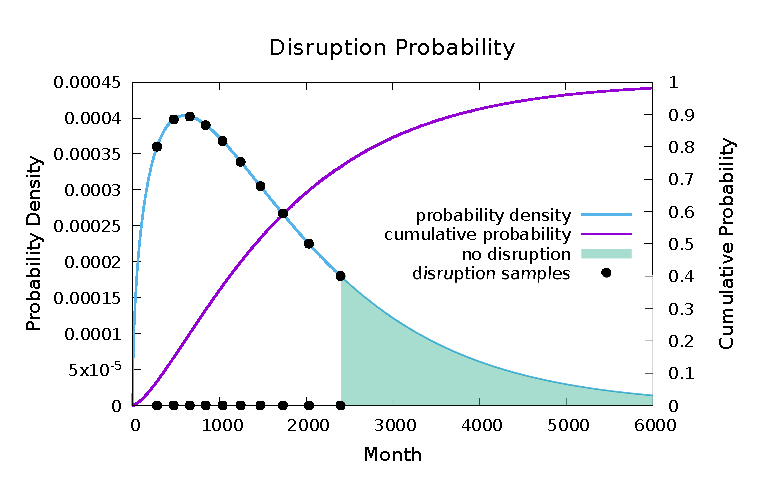
\includegraphics[width=1.0\columnwidth]{gamma-dist.eps}
    \caption[Disruption Probability Distribution]{
        The disruption probability density function is a scaled gamma
        distribution (i.e. Equation \ref{eq:gamma-dist}).  Note that the
        simulation duration is 2,400 months; times after month 2,400 are
        beyond the planning horizon and represent no disruption occurring.
    }
    \label{fig:exp3-gamma-dist}
\end{figure}


\subsubsection{Results}

This problem was used to demonstrate the hedging strategy analysis.
Intermediate results were used to assess the impact of the assumptions
inherent in this analysis and are analyzed more comprehensively in
Ref. x\citeprod{rwc-dissertation}.  To assess the quality of the best hedging
deployment history identified by this methodology, it is useful to compare its
performance to other possible deployment histories.  In addition to comparing
the value of $H(D)$ for different deployment histories, it is valuable to
consider the probability distribution functions (PDFs) of objective function
values, over a large set of randomly sampled disruption times.


Figure \ref{fig:exp3-outcome-dists} shows the PDFs for the hedging strategy
compared to 6 other deployment histories, specifically the best deployment
strategies for 6 different fixed/known disruption times.  It is apparent that
a number of deployment histories have lower objective function values in their
best case than the best case for the hedging strategy, but may also have a
higher prevalence of higher objective function values.

\begin{figure}[!htb]
    \centering
    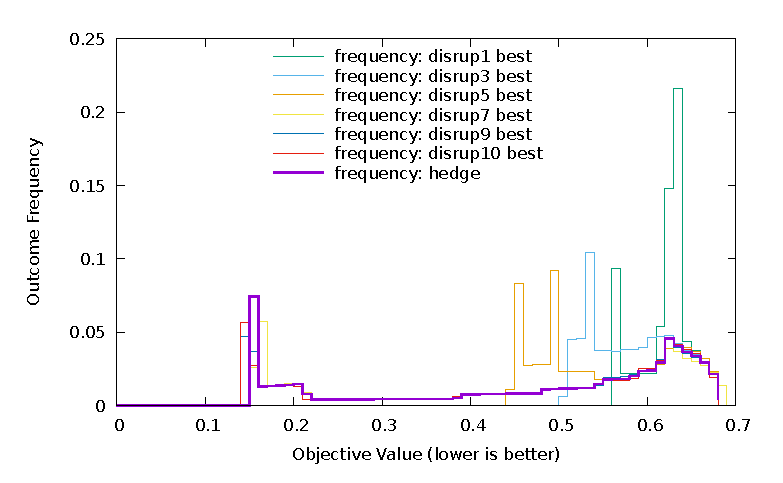
\includegraphics[width=1.0\columnwidth]{dists.eps}
    \caption[Outcome Distributions in Hedging Analysis]{
        The best deployment schedules from select disruption times and the
        hedging schedule were used in to sample disruption times from the PDF.
        Best achievable objectives were then collected and the outcome
        frequency for each is shown.  Better hedging strategies shift more
        outcomes to the left toward better values (e.g. hedge, disruption 10,
        etc.).  The 26.1\% no-disruption probability causes a spike of
        outcomes all at the left/lower edge of each distribution curve.
        Because this obscures other data, the no-disruption outcomes are
        omitted from the plot.
    }
    \label{fig:exp3-outcome-dists}
\end{figure}


\subsubsection{Summary}

Because of the black-box nature of the \Cyclus optimization system, it was
possible to extend it to a nested optimization system by changing the
mechanism for evaluating the objective function.  In a typical scenario
optimization, a single objective function evaluation is a single \Cyclus{}
simulation with some post processing.  For the hedging analysis, using an
approximation at one layer of the nested optimization, a single objective
function evaluation is $O(10)$ \Cyclus simulations that are combined into a
single value.  This methodology was demonstrated using a posited disruption
to the EG23 transition scenario, identifying a the best deployment history for
minimizing the exposure to that disruption.


\section{Summary}

This project identified two primary goals related to the introduction of
optimization capability into the \Cyclus{} fuel cycle simulation ecosystem:
\begin{enumerate}
\item optimization at the market-level for individual commodity trades at each time step, and 
\item optimization at the system-level to identify the best deployment
  histories over a fuel cycle transition.
\end{enumerate}
\noindent Both of these goals were successfully accomplished with minor variations from
orignially proposed research plan.

\subsection{Market-level Optimization}

The mechanism for matching resource requests made by some facilities with
resource offers made by other facilities was finalized and implemented as a
variation of a classic network transportation problem.  Specific additions
were made to account for the fungibility of some nuclear materials, the desire
for exclusive supply arrangements, and the possibility for constraints that
are functions of both resource quality and quantity.  This approach also
preserves the important feature of retaining full agency within each facility
for determining its preference among the offers that can satisfy its requests.

The specific task of assessing different optimization algorithms was completed
with a comprehensive comparison of a fast heuristic market matching algorithm
with more rigorous linear programming algorithms provided by \gls{COIN-OR}.
The heuristic matching algorithm was found to be sufficient in many cases,
although it is not yet clear how to determine that it will be sufficient for
any particular problem.  Although the total objective function value of
different material flow solutions may vary, such variations do not always
represent substantially different flows.

The specific task of introducing objective function callbacks to allow
suppliers to detremine what preference each consumer will assess for its
offers, and therefore tailor the offers to maximize the likelihood of
matching.  This feature both adds efficiency to the market mechanisms by
improving the quality of individual offers and/or reducing the total number of
offers necessary to reach an optimal solution.

The single deviation from the orignial research plan was that realistic
economic value functions were not implemented in place of preference.  While
it is possible for each facility archetype to rely on realistic economic
values to assess its preference for individual trades, insufficient certainty
in economic models exists to justify incorporating this in specific facility
archetypes being delivered formally as part of the \Cyclus{} ecosystem.

\subsection{System-level Optimization}

A system for seeking and identifying optimal deployment histories was
developed based on black-box optimization techniques.  A PSwarm algorithm was
found to be the most effective at converging on optimal deployment histories,
following comparison with a variety of open source algorithms that satisfied
the requirements for optimization of this kind of problem.  The formulation of
the decision space was found to be important to improve the rate of
convergence.  A master-worker paradigm was implemented to take advantage of
high throughout and/or cloud computing resources necssary to accompish the
$O(10^5)$ \Cyclus{} simulations necessary in this kind of optimization.

The optimization system was demonstrated using the EG23 fuel cycle transition
defined by the Fuel Cycle Options campaign.  While the FCO campaign relied on
manual iteration to identify an optimum deployment history, the optimization
system was able to automatically arrive at an equivalent deployment history.
Allowing for some flexibility in the overall power constraint allowed the
system to find a more optimal solution that completes the transition more
quickly.

One contribution beyond the original research plan was to use this
optimization system to compare the impacts of different modeling choices,
namely the difference between modeling indviidual facilities and fleets of
facilities, and the difference between 1 month and 3 month time
steps. \citeprod{rwc_fleet}

One substantinal contribution beyond the original research plan was the
adaptation of the optimization system for identifying hedging strategies in
the face of possible disruptions to the planned fuel cycle transition.  A
conceptual methodology was designed that relies on nested optimization, and
implemented with an approximation to one level of optimization to reduce the
overall computational burden to a reasonable level.






%% 4. Provide a comparison of the actual accomplishments with the goals and
%%    objectives of the project.


%% 6. Identify products developed under the award and technology transfer activities, such as:
%%    a. Publications (list journal name, volume, issue), conference papers, or
%%       other public releases of results. If not provided previously, attach or
%%       send copies of any public releases to the DOE Program Manager identified
%%       in Block 15 of the Assistance Agreement Cover Page;
%%    b. Web site or other Internet sites that reflect the results of this
%%       project;
%%    c. Networks or collaborations fostered;
%%    d. Technologies/Techniques;
%%    e. Inventions/Patent Applications, licensing agreements; and
%%    f. Other products, such as data or databases, physical collections, audio
%%       or video, software or netware, models, educational aid or curricula,
%%       instruments or equipment.


\end{document}

%% Final Scientific/Technical Report

%% Content. The final scientific/technical report must include the following
%% information and any other information identified under Special Instructions on
%% the Federal Assistance Reporting Checklist:


%% 5. Summarize project activities for the entire period of funding, including
%%    original hypotheses, approaches used, problems encountered and departure
%%    from planned methodology, and an assessment of their impact on the project
%%    results. Include, if applicable, facts, figures, analyses, and assumptions
%%    used during the life of the project to support the conclusions.



%% 7. For projects involving computer modeling, provide the following information
%%    with the final report:
%%    a. Model description, key assumptions, version, source and intended use;
%%    b. Performance criteria for the model related to the intended use;
%%    c. Test results to demonstrate the model performance criteria were met
%%       (e.g., code verification/validation, sensitivity analyses, history
%%       matching with lab or field data, as appropriate);
%%    d. Theory behind the model, expressed in non-mathematical terms;
%%    e. Mathematics to be used, including formulas and calculation methods;
%%    f. Whether or not the theory and mathematical algorithms were peer
%%       reviewed, and, if so, include a summary of theoretical strengths and
%%       weaknesses;
%%    g. Hardware requirements; and
%%    h. Documentation (e.g., users guide, model code).

%% Electronic Submission. The final scientific/technical report must be submitted
%% electronically via the DOE Energy Link System (E-Link) accessed at
%% http://www.osti.gov/elink-2413.

%% Electronic Format. Reports must be submitted in the ADOBE PORTABLE DOCUMENT
%% FORMAT (PDF) and be one integrated PDF file that contains all text, tables,
%% diagrams, photographs, schematic, graphs, and charts. Materials, such as
%% prints, videos, and books, that are essential to the report but cannot be
%% submitted electronically, should be sent to the DOE Administrator at the
%% address listed in Block 16 of the Assistance Agreement Cover Page.

%% Submittal Form. The report must be accompanied by a completed electronic
%% version of DOE Form 241.3, “U.S. Department of Energy (DOE), Announcement of
%% Scientific and Technical Information (STI).” You can complete, upload, and
%% submit the DOE F.241.3 online via E-Link. You are encouraged not to submit
%% patentable material or protected data in these reports, but if there is such
%% material or data in the report, you must: (1) clearly identify patentable or
%% protected data on each page of the report; (2) identify such material on the
%% cover of the report; and (3) mark the appropriate block in Section K of the
%% DOE F 241.3. Reports must not contain any limited rights data (proprietary
%% data), classified information, information subject to export control
%% classification, or other information not subject to release. Protected data is
%% specific technical data, first produced in the performance of the award that
%% is protected from public release for a period of time by the terms of the
%% award agreement. '
